\documentclass[12pt]{article}
%%%%%%%%%%%%%%%%%%%%%%%%%%%%%%%%%%%%%%%%%%%%%%%%%%%%%%%%%%%%%%%%
%%  LaTeX Preamble
%%  Comiple using "LuaTeX" the successor to pdfTeX
%%%%%%%%%%%%%%%%%%%%%%%%%%%%%%%%%%%%%%%%%%%%%%%%%%%%%%%%%%%%%%%%
\usepackage{letterhead-UD}  % Nick's UD letterhead stylesheet
%-----------------------------------------------------------------------
\usepackage{amsmath}
\usepackage{unicode-math}
\setmainfont{EB Garamond}
\setmathfont{Garamond-Math.otf}[StylisticSet={8,9}]
% If you want a script-style \mathscr in addition to
% the calligraphic-style \mathcal, add:
\setmathfont{Garamond-Math.otf}[range={scr,bfscr}]

%%%%%%%%%%%%%%%%%%%%%%%%%%%%%%%%%%%%%%%%%%%%%%%%%%%%%%%%%%%%%%%%
%%  LaTeX Preamble
%%%%%%%%%%%%%%%%%%%%%%%%%%%%%%%%%%%%%%%%%%%%%%%%%%%%%%%%%%%%%%%%
\usepackage[explicit]{titlesec} % interface to sectioning commands
\usepackage[shortlabels]{enumitem}
\usepackage{tabularx}
\usepackage{graphicx}
\usepackage{svg}
\usepackage{lipsum}
\usepackage{outlines}
\usepackage{deepoutline}         % https://tex.stackexchange.com/questions/262721/increasing-the-maximum-number-of-enumerate-environments
\usepackage{tabularray}          % use LATEX3 functions to parse the table, and then typeset the entire table
\usepackage{pifont}              % Provides access for Pi fonts (Dingbats, Symbols, etc)
\usepackage{xspace}
\usepackage{fontawesome5}
\usepackage{hyperref}
\hypersetup{
    colorlinks=true,
    linkcolor=red2,
    filecolor=magenta2,      
    urlcolor=azure2,
    }
%%%%%%%%%%%%%%%%%%%%%%%% Bib STUFF %%%%%%%%%%%%%%%%%%%%%%%%%%%%%
\usepackage[style=ieee,backend=biber,dashed=false,doi=false,eprint=false, sorting=nyt]{biblatex}
\addbibresource{main.bib}
% Nick wants ??? back
\makeatletter
\def\abx@missing@entry#1{\abx@missing{??}}
\makeatother

%%%%%%%%%%%%%%%%%%%%%%%%%%%%%%%%%%%%%%%%%%%%%%%%%%%%%%%%%%%%%%%%
\pagestyle{fancyplain}
%%%%%%%%%%%%%%%%%%%%%%%%%%%%%%%%%%%%%%%%%%%%%%%%%%%%%%%%%%%%%%%%%
% section Stuff
%%%%%%%%%%%%%%%%%%%%%%%%%%%%%%%%%%%%%%%%%%%%%%%%%%%%%%%%%%%%%%%%%
\renewcommand{\thesection}{\arabic{section}}
\renewcommand{\thesubsection}{\thesection.\Alph{subsection}}


\newlength{\seclength}
\settowidth{\seclength}{00.\hspace*{.5em}}
\titleformat{\section}
  {\normalfont\large\bfseries}  % The style of the subsection title
  {\makebox[\seclength][l]{\thesection.}}                            % a prefix
  {.25em}                         % space between prefix and title
  {\textsc{#1}}          % How the section is represented

\newlength{\sseclength}
\titleformat{\subsection}[block]
  {\normalfont\normalsize\large\itshape\bfseries}  % The style of the subsection title
  {}                         % a prefix
  {0pt}                        % space between prefix and title
  {\uline{\textsc{#1}}} % How the section is represented
  %{\uline{\MakeUppercase{#1}}} % How the section is represented

\titleformat{\subsubsection}[block]
  {\hspace*{36pt}\normalfont\normalsize\bfseries}  % The style of the subsection title
  {}                            % a prefix
  {0pt}                         % space between prefix and title
  {#1}                          % How the section is represented

% Section spacing: Left before after right
\titlespacing{\section}{0pt}{6pt plus 2pt minus 1pt}{3pt plus 2pt minus 1pt}
% Subsection spacing: Left before after right
\titlespacing{\subsection}{0pt}{3pt plus 2pt minus 1 pt}{2pt plus 2pt minus 1pt}
% Sub-subsection spacing: Left before after right
\titlespacing{\subsubsection}{0pt}{1pt plus 2pt minus 1 pt}{1pt plus 1pt minus 1pt}
%%%%%%%%%%%%%%%%%%%%%%%%%%%%%%%%%%%%%%%%%%%%%%%%%%%%%%%%%%%%%%%
% Commands
%%%%%%%%%%%%%%%%%%%%%%%%%%%%%%%%%%%%%%%%%%%%%%%%%%%%%%%%%%%%%%%
\newcommand{\xmark}{\text{\ding{55}}}%
\newcommand{\cmark}{\text{\ding{51}}}%
\def\labelitemi{\footnotesize\ding{108}}
\def\labelitemii{\small\ding{228}}
\def\labelitemiii{\tiny\ding{109}}
\def\labelitemiv{\tiny\ding{226}}

\newcommand*\chk{\item[\checkmark]}
\newcommand*\arr{\item[\faIcon{angle-right}]}

\newcommand{\scl}[1]{\begin{itemize} \chk #1 \end{itemize}}  % single item list
\newcommand{\sal}[1]{\begin{itemize} \arr #1 \end{itemize}}  % single item list

\NewDocumentCommand{\boldd}{m}{\textbf{\$}$\mathbf{#1}$}
%\NewDocumentCommand{\scriptr}[1]{\ensuremath{\mathcalligra{#1}}}
\NewDocumentCommand{\soe}{}{School of Engineering\xspace}
\NewDocumentCommand{\college}{}{College of Arts \& Sciences\xspace}

%%%%%%%%%%%%%%%%%%%%%%%%%%%%%%%%%%%%%%%%%%%%%%%%%%%%%%%%%%%%%%%
% Header info
%%%%%%%%%%%%%%%%%%%%%%%%%%%%%%%%%%%%%%%%%%%%%%%%%%%%%%%%%%%%%%%
%\title{Directing the Narrative:\protect\\eliciting observable behavior for agent classification}
% \title{Real-Time Closed-loop Control for Additive Manufacturing }
% \title{\vspace{-1.59cm}Neural Network-based Closed-loop Control of LPBF-AM Process with Multimodal Sensor Fusion \vspace{-2ex}}

\title{\vspace{-1.59cm}Multi Modal Sensor Fusion for Closed-loop Control for Additive Manufacturing \vspace{-2ex}}

%Eliminating LPBF-AM Part Defects through Neural Network-Based Closed-Loop Control and Multimodal Sensor Fusion

%Enhancing LPBF-AM Process Precision through Neural Network-Based Closed-Loop Control and Multimodal Sensor Fusion
%Optimizing Laser Powder Bed Fusion Additive Manufacturing: Advanced Neural Networks and Multimodal Sensor Fusion for Precision Closed-Loop Control
% Real-Time Closed-Loop Control of LPBF-AM Process with Multimodal Sensor Fusion
\author{Abdullah A Amin and Krishna B Kidambi \protect\\ 
Department of Mechanical and Aerospace Engineering, University of Dayton \vspace{-2ex}}
\date{}
%%%%%%%%%%%%%%%%%%%%%%%%%%%%%%%%%%%%%%%%%%%%%%%%%%%%%%%%%%%%%%%%
% Begin Document
%%%%%%%%%%%%%%%%%%%%%%%%%%%%%%%%%%%%%%%%%%%%%%%%%%%%%%%%%%%%%%%%
\begin{document}
\maketitle
\NineColors{saturation=high}
% \textbf{Intellectual Merit:}
The objective of the proposed research is to integrate Dempster-Shafer theory with neural networks (NN) for multi-modal sensor fusion (infrared, ultrasound, eddy current) for real-time closed-loop feedback control to improve part quality in additive manufacturing (AM). Utilizing publicly available open-source sensor data by National Institute of Standards and Technology (NIST) and Airforce Research Laboratory (AFRL) in combination with simulation data generated using PIs award-winning AM computational solver, multi-modal data will be generated for sensor fusion. This hybrid data generation method will serve as the ground truth for designing feedback control algorithms. Finally, based on the ground truth, a robust adaptive control technique will be developed to regulate the AM process parameters in real-time, thereby ensuring the production of defect-free components.

\begin{outline}[enumerate]
    \1 Develop ground truth data utilizing the open-source experimental and generate simulated data using state of the art AM solvers. 
    \1 By utilizing Dempster-Shafer theory and amalgamating with NN, develop sensor fusion techniques to reduce uncertainty in individual sensor modalities.
    \1 Develop closed-loop (robust and adaptive) control techniques to adjust the laser power, spot diameter, scan speed  to minimize different types of porosities in metal AM parts.
\end{outline}
% In the rapidly evolving landscape of additive manufacturing (AM), achieving precision, repeatability, and quality in produced parts requires sophisticated sensory and control mechanisms. The advent of increased computational capabilities, coupled with advancements in sensing technology, has propelled feedback control to the forefront of modern manufacturing processes. The AM research community focused on monitoring and controlling various process variables such as molten pool width and temperature, laser power and focus, scan and powder feed speed to name a few.
%
% Traditional cameras (CMOS, infrared and digital) and ultrasound sensors have been used to measure layer height, geometric accuracy and cooling rates. Conventional strategies like transfer function approach, PID and nonlinear approaches like Sliding mode control have been implemented for closed-loop feedback control of AM processes. These techniques have been prevalent in recent years and have yielded successful results (reducing the process time and roughness, repeatability). But many mature AM systems only sense and control single geometrical features. 
%
% The objective of this proposed research is to integrate Dempster-Shafer theory with Neural Network to fuse multiple sensor data (infrared, ultrasound, eddy current) specific to metal Additive Manufacturing machines for improved part quality. There are publicly available sensor data shard by National Institute of Standards and Technology (NIST) and handful or other researchers around the world. In addition, the PIs will generate simulation data by an award winning AM computational solver. These experiment and simulation data provided as ground truth (Objective 1) in combination with multimodal sensor data will be key input to the Dempster-Shafer based neural network to generate comprehensive understanding (Objective 2) and response of the AM process in real time. Based on the outcome and with the help of the robust adaptive controller, the laser power, spot diameter, scan speed will be adjusted in real time to control two different types of porosites in metal AM parts, i. lack of fusion, ii. keyhole porosities (Objective 3). 

\begin{figure}[htbp]
  \centering
  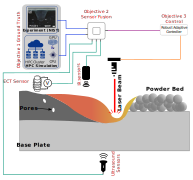
\includegraphics[width=0.51\textwidth]{figures/SensorFusion.png}
  % \includesvg[width=1\textwidth]{figures/SensorFusion.svg}
  \caption{Concept of sensor fusion for metal additive manufacturing.}
  \label{fig:labelForYourFigure}
\end{figure}

% In order to mitigate the above mentioned challenges, in this proposal we aim to investigate the following objectives: 
% \begin{outline}[enumerate]
% \1 Develop fusion models between multiple sensing modalities (IR thermography, Ultrasound, x-ray synchrotron) and develop robust control techniques in myriad of control situations (over actuated and under actuated)
% % Multi-information fusion algorithms or fusion models based on multi-sensor systems to achieve higher accuracy and stronger robustness.
% % \1 Train a physics-informed machine learning models based on available test data combined with thermo-fluid PDEs solutions for AM problem, next use the network for closed-loop control operation to ensure reduced defect/defect free AM parts. 
% \1 Train a physics-informed machine learning models based on available test data combined with thermo-fluid PDE solutions for AM problem to extract the relationship between process parameters and the controlled variables. 
% \1 Establish validation metrics under uncertainties in both process and controlled variables by using trained network to predict the corrective action in a closed-loop control setting to ensure reduced defect/defect free AM parts.
% % \1 Develop machine learning algorithms to extract the relationship between process parameters and geometrical features. 
% \end{outline}
\section*{Intellectual Merits}
This research will help reduce defects in the metal AM parts, resulting in improved material properties and superior fatigue performance. The successful development of the innovative sensor fusion techniques will help accelerate the metal AM technologies to replace the conventional manufacturing processes. These advancements will not only reduce material waste, promoting more sustainable manufacturing practices, but also bolster U.S. manufacturing capabilities and decrease reliance on foreign resources. 

\section*{Broader Impact}
The proposed research plans to train high school, undergraduate, graduate, and postdoctoral scholars in additive manufacturing and prepare them for the future workforce. The plan to support these future STEM professionals is through a high school summer program, research experience for undergraduate (REU), graduate student support, and postdoctoral research opportunities. Disseminating the research outcome would consider wide range of media for education and training such as scientific journal articles, workshops, podcasts, social media platforms. An advanced graduate-level course will also be developed as part of the knowledge-creation plans. Establishing collaborations with local industry partners will facilitate an effective means for technology transfer and stimulating economic growth.
\end{document}

